\documentclass[12pt]{ctexart} % 使用 ctexart 文档类支持中文

\usepackage{fancyhdr} % 奇特的 header
\usepackage{xcolor} % 更多颜色

\usepackage[utf8]{inputenc} % 支持 UTF8 字符,在 UTF8 engine 中无需此行
\usepackage{xeCJK} % 支持中文排版,已经包含在 ctexart 中
\usepackage{fontspec} % 字体设置
\usepackage{geometry} % 页面布局
\usepackage{titlesec} % 自定义标题样式
\usepackage{setspace} % 设置行距
\usepackage{microtype} % 更多的微调
\usepackage{tabularx} % 表格支持

\usepackage{float} % Add the float package,支持图片位置固定

\usepackage[colorlinks,linkcolor=black,urlcolor=black]{hyperref} % 超链接支持

\usepackage{tocloft} % 自定义目录样式

\usepackage{graphicx} % 图片设置
\graphicspath{ {./images/} }

% 设置页面布局
\geometry{a4paper, margin=1in}

% 设置行距为 1.25 倍
\setstretch{1.25}

% 设置中文字体
\setCJKmainfont{SimSun}[BoldFont={Microsoft YaHei Bold}] % 设置正文为宋体

\setCJKsansfont{Microsoft YaHei}[BoldFont={Microsoft YaHei Bold}] % 标题等无衬线字体为黑体

% 设置英文字体
\setmainfont{Times New Roman}



% 配置页眉和页脚
\pagestyle{fancy}
\fancyhf{}

\renewcommand{\headrulewidth}{0pt}

\setlength{\headheight}{25.60938pt} % Set the headheight to the required value
\addtolength{\topmargin}{-13.60938pt} % Adjust the topmargin to compensate

% 定义颜色
\definecolor{myblue}{RGB}{152, 220, 222} % 蓝色

% 左侧页眉设置, 页码在页眉外侧
\fancyhead[L]{%
  \colorbox{myblue}{%
    \parbox[t]{1cm}{%
      \textcolor{white}{\thepage}%
    }%
  }%
  \hspace{0.5cm}
  总体设计报告
}

% \fancyhead[L]{\leftmark} % 左页显示章节名

% 页眉横线设置
\renewcommand{\headrulewidth}{0.5pt}
\renewcommand{\headrule}{%
  \hbox to\headwidth{%
    \color{black}\leaders\hrule height \headrulewidth\hfill%
  }%
}

% 页脚页数设置
\renewcommand{\footrulewidth}{0pt}
\fancyfoot[C]{\thepage}

% 设置目录样式
\renewcommand{\cftsecfont}{\bfseries} % 目录中章节标题加粗

\titleformat{\section}
  {\normalfont\Large\bfseries} % 移除 \centering
  {\thesection}{1em}{}


% 超链接设置
\hypersetup{
  colorlinks=true,
  linkcolor=black,
  filecolor=magenta,      
  urlcolor=cyan,
}


\begin{document}

\begin{titlepage}
  \centering % 居中对齐
  % \vspace*{1cm} % 从顶部添加一些垂直间距
  
\includegraphics[width=0.6\textwidth]{zjutitle.jpg} % 插入图片
  
  \vspace{2cm} % 添加垂直间距
  
  {\fontsize{36}{48}\selectfont\CJKfontspec{Microsoft YaHei} 总体设计报告} % 标题
  
  \vspace{2cm} % 添加垂直间距
  
  
\includegraphics[width=0.4\textwidth]{zjulogo.jpg} % 插入图片
  
  \vspace{2cm}
  
  {\Huge\CJKfontspec{Microsoft YaHei} 项目主题: \underline{H5游戏分享平台}} % 项目主题 with underline
  
  \vspace{1cm}

  {\Large\CJKfontspec{Microsoft YaHei} 第 1 小组: \underline{肖一鸣、金谞健、马宇恒、杨仕平、周睿}} % 作者
  
  \vspace{1cm} % 添加垂直间距
  
  {\Large\CJKfontspec{Microsoft YaHei} \today} % 日期

\end{titlepage}

\newpage
\tableofcontents % 自动生成目录
\newpage

\section{体系结构设计}

\subsection{体系结构风格}
在软件工程中,体系结构风格是用于定义软件系统高层次结构和组织模式的抽象框架。它是一种通用的、可复用的解决方案,
用于在特定上下文中组织软件系统的结构与交互方式,描述了系统组件的类型、组件间的交互方式、约束条件以及适用的场景,为设计决策提供指导原则。

一个体系结构风格通常包括:
组件类型(系统由哪些功能模块组成),连接件类型(模块之间如何通信),
拓扑结构(组件和连接件的组织方式),语义约束(对交互方式、数据流动、控制流的限制)。

体系结构风格是设计系统的“蓝图”,选择时需要权衡利弊,结合具体场景灵活应用。
为了找到适合我们软件的体系结构风格,我们参考了以下常见的体系结构风格。

\subsubsection{以数据为中心的体系结构}
在以数据为中心的体系结构(Data‑Centric Architecture)中,数据是系统的核心枢纽,所有功能组件都围绕这个中心进行设计与交互。
它的核心概念是:拥有一个一个全局可见的数据存储(称为中心存储),负责持久化并管理系统的“真相版本”;
各类模块都不直接相互通信,而是通过读写中心存储完成信息交换;
为了保证各方都能正确理解和操作数据,需要设计一致且规范化的元数据模型。

以数据为中心的架构通常涉及以下组件:
\begin{itemize}
  \item 中央数据存储:

  作为系统的“唯一数据源”,存储所有结构化或非结构化数据。要支持高并发读写、数据持久化和一致性。
  \item 数据访问层:
  
  提供统一的接口供其他组件访问数据,隐藏底层存储细节,标准化数据访问权限,提升安全性。
  \item 数据处理引擎:
  
  负责数据的清洗、转换、分析和计算,支持实时或离线数据处理。
  \item 数据总线或消息队列:
  
  实现数据的异步传输和组件间解耦,支持高吞吐量、低延迟的数据流动。
  \item 元数据管理:
  
  记录数据的定义、来源、格式、血缘关系等上下文信息,确保数据可发现、可理解、可追溯。
  \item 客户端/应用接口:
  
  供用户或外部系统与数据交互,可以包括用户界面、网页或API等组件。 
  \item ETL/ELT工具(数据集成):
  
  从外部系统抽取(Extract)、转换(Transform)、加载(Load)数据到中央存储。
\end{itemize}

以数据为中心的体系结构通过将数据存储作为枢纽,解耦了各功能模块、统一了数据视图,
特别适合需要共享、可审计、可追溯的大型系统与大数据平台。
但它对存储系统的可用性、可扩展性和数据治理提出了较高要求。

\subsubsection{数据流体系结构}
数据流(Data Flow)体系结构是一种以数据流动为中心组织系统的软件架构风格,它将系统功能分解为一系列独立的处理单元(过滤器),
通过“管道”将数据从一个单元传递到下一个单元。整个系统的数据流向决定了组件的执行顺序和交互方式。

数据流体系结构通常涉及以下组件:
\begin{itemize}
  \item 数据源:

  生成或提供原始数据,是数据流的起点。常见的有传感器、数据库、消息队列、API接口等。
  \item 数据处理单元:
  
  对数据进行转换、计算或过滤,每个单元负责单一功能。常见的有过滤器、聚合器、分析器等。
  \item 管道:
  
  连接数据处理单元,负责数据传输,确保数据有序流动。可以是单向或双向,可能包含缓冲区。
  \item 数据接收器:
  
  存储或展示处理后的最终结果,通常以数据库、文件系统形式出现。
  \item 控制逻辑:
  
  协调数据流的方向、优先级或错误处理。需要实现路由规则,有容错机制。
  \item 数据缓冲区:
  
  临时存储数据,解决生产者-消费者速度不匹配问题。如在高吞吐量数据流中防止数据丢失或阻塞。
\end{itemize}

数据流体系结构强调“数据即主角”,通过把处理逻辑拆分成一系列可复用的过滤器,并以管道将它们串联起来,
实现了高内聚低耦合、易扩展与并行的系统设计。适用于实时流处理、信号处理等场景。

\subsubsection{调用和返回体系结构}
调用-返回(Call-and-Return)是一种经典的体系结构风格,也常被称为过程式或分层分解风格。
它的核心思想是将系统划分为若干模块(组件),模块之间通过子程序(或函数)的调用和返回来协作和传递控制权。

调用和返回体系结构通常涉及以下组件:
\begin{itemize}
  \item 主程序:

  作为系统的入口点和总控制器,负责协调子程序或模块的调用顺序。
  通常是程序的起点(如main函数),负责初始化系统资源(如内存、配置文件)。
  \item 子程序/函数:
  
  封装特定功能的可重用代码块,通过调用触发执行,通过返回传递结果。
  可以是过程(无返回值)或函数(有返回值)。支持参数传递和局部变量。
  \item 模块:
  
  将相关子程序组织成逻辑单元(如代码文件、库),实现功能隔离和高内聚。
  通常通过接口(如头文件)暴露功能,隐藏实现细节。
  \item 调用栈:
  
  管理函数调用和返回的执行上下文,记录当前执行位置、参数和局部变量。
  采用后进先出(LIFO)结构,确保函数返回时能恢复之前的执行状态。
  \item 返回机制:
  
  子程序执行完毕后,将结果和控制权交回调用者。
  \item 控制模块:
  
  在复杂系统中用一个专门的模块负责调度子程序的调用顺序。类似状态机或调度器,根据条件动态选择调用的子程序。
\end{itemize}

它的优势在于易于理解和实现,符合大多数编程语言的执行模型,并且调试方便,功能清晰且模块化。
但他也有着层间耦合严重,跨层修改困难,可扩展性有限,不适合高度动态或分布式场景等问题。

\subsubsection{面向对象体系结构}
面向对象体系结构(Object‑Oriented Architecture)是一种基于面向对象思想来组织系统结构的架构风格。
它将系统划分为松耦合的“对象”单元,通过对象之间的消息传递来协作,实现高内聚、可扩展和可重用的目标。

面向对象体系结构通常涉及以下组件:
\begin{itemize}
  \item 类:

  类是对象的蓝图,定义了对象的属性(数据)和方法(行为)。
  能够封装数据和行为,隐藏实现细节,并支持继承和多态。
  \item 对象:
  
  对象是类的实例,是系统中运行时的基本操作单元,
  通过消息传递(方法调用)与其他对象交互。
  \item 接口:
  
  接口是行为的抽象契约,定义了一组方法签名,但不提供具体实现。
  它实现了多态和松耦合,支持“面向接口编程”,并允许多个类通过实现同一接口提供不同行为。
  \item 关系:
  
  面向对象体系结构通过继承、组合、聚合、依赖等关系组织组件。
  \item 设计模式:
  
  设计模式是面向对象体系结构中解决常见问题的可复用方案,例如工厂模式、观察者模式等等。
  \item 框架:
  
  框架是面向对象体系结构的半成品实现,提供基础结构和扩展点。
\end{itemize}

它有着高内聚、低耦合,可扩展性强,重用性好,易于映射到现实世界等优势,
适用于业务逻辑复杂、对象之间交互频繁的系统或者是需要频繁迭代、功能不断扩展的长期维护项目。
但它的性能开销与较高的设计门槛成为了它的局限。

\subsubsection{层次体系结构}
层次体系结构(Layered Architecture)是一种将系统划分为若干“层”(layer)的架构风格,
每一层只与它的上下邻近层发生交互,从而实现关注点分离、模块化和松耦合。

层次体系结构通常涉及以下核心层(经典的三层架构):
\begin{itemize}
  \item 表现层:

  处理用户交互和界面展示,包含UI、控制器、视图模板等组件。
  \item 业务逻辑层:
  
  实现系统的核心业务规则和流程。包含服务、领域模型、事务管理等组件。
  \item 数据访问层:
  
  负责与数据源(如数据库、外部API)交互。
  包含了数据访问对象(Data Access Object)、ORM框架、数据库连接池等组件。
\end{itemize}

它有着关注点分离、可替换性、团队并行开发等优势,适用于业务逻辑复杂、模块众多的中大型企业应用。
但会出现新跟那个开销大,不恰当的层次依赖等问题。

\subsubsection{客户端-服务器架构}
客户端-服务器(Client–Server)架构是一种最常见的软件体系结构模式,核心思想是将系统划分为两类角色:
\begin{enumerate}
  \item 客户端(Client):

  发起请求的一方,通常运行在用户终端,负责处理用户界面、输入校验、本地缓存等,
  会向服务器发送服务请求,并接收、呈现服务器返回的数据。
  \item 服务器(Server):
  
  接收并处理客户端请求,执行核心业务逻辑、访问数据库、调用第三方服务等。
  会将处理结果(通常是数据)返回给客户端。
\end{enumerate}

客户端-服务器架构通常涉及以下组件(上面已经提到的客户端和服务器省略):
\begin{itemize}
  \item 网络基础设施:

  客户端和服务器的交互依赖底层网络组件,如通信协议、负载均衡器、防火墙与安全组件等。
  \item 中间件与辅助组件:
  
  在复杂系统中,可能需要更多的支持性组件,
  如缓存服务器、消息队列、API网关、日志与监控系统等等。
\end{itemize}

客户端‑服务器架构以其清晰的职责划分和成熟的通信机制,成为现代应用系统的主流模式。
在此基础上,通过多层拆分、缓存、负载均衡、异步消息等技术,可构建高可用、高性能、易扩展的分布式系统。
它适用于绝大多数互联网应用、企业内部系统以及移动应用的后端。

\subsubsection{浏览器-服务器架构}
浏览器–服务器(Browser–Server,简称 B/S)架构是一种典型的客户端–服务器(C/S)变体,专门针对 Web 应用场景而设计。
其核心思想是把表示层完全放在浏览器端,服务器端只负责业务逻辑和数据存储。

浏览器-服务器架构通常涉及以下组件:
\begin{itemize}
  \item 客户端(浏览器):

  它是用户与系统交互的界面,负责发送请求、接收响应并渲染内容。
  关键功能在于解析并展示HTML/CSS/JavaScript内容,以及管理Cookie、本地存储等。
  \item 服务器端组件:
  
  通常由多个层次,如接收HTTP请求、返回静态资源或转发动态请求的Web服务器,
  处理业务逻辑、生成动态内容的应用服务器,持久化存储业务数据的数据库等
  \item 网络协议:

  主要是HTTP/HTTPS,它们是浏览器与服务器通信的基础协议,HTTPS通过SSL/TLS加密确保安全。
  \item 中间件:

  这部分虽然可选,但也比较常见。例如用于负载均衡、安全过滤的反向代理,还有缓存服务器,消息队列,内容分发网络等等。
  \item 安全组件:

  包含过滤恶意流量的防火墙,确保HTTPS通信加密的SSL证书,还有认证服务以及日志等。
\end{itemize}

它有着零客户端安装、跨平台、易于部署与更新、扩展性好等优势,适用于各种网站的开发。
但它的服务器性能瓶颈、HTTP的安全风险以及前后端耦合的问题成为了它的局限。

\subsubsection{微服务架构}
微服务架构(Microservices Architecture)是一种将单一应用拆分为一组小型、独立部署服务的架构风格。
每个微服务围绕业务能力构建,可独立开发、测试、部署和扩展,并通过轻量级通信机制相互协作。

微服务架构通常涉及以下组件:
\begin{itemize}
  \item 微服务:

  独立的服务单元,每个服务负责一个特定的业务功能(如用户管理、订单处理)。
  能独立开发、部署和扩展,并可以使用不同的技术栈。
  \item API网关:
  
  作为系统的统一入口,负责路由请求、协议转换、身份验证、限流等。
  关键在于将客户端请求路由到对应的微服务,并聚合多个服务的响应以及实施安全策略。
  \item 服务发现与注册中心:

  动态管理服务的地址和状态,实现服务间的自动发现。
  \item 配置中心:

  集中管理所有微服务的配置(如数据库连接、环境变量),支持动态更新。
  能够避免硬编码配置,简化多环境(开发、测试、生产)管理。
  \item 其他:

  除上述提到的之外,还有通信组件,数据管理组件,安全组件,事件总线等等。
\end{itemize}

微服务架构能够显著提高系统的可扩展性、可维护性和团队交付效率,但也带来分布式治理、数据一致性和运维自动化的额外复杂度。
尝试时应结合团队规模、业务复杂度及技术栈成熟度,切实完善配套能力。

\subsubsection{事件驱动架构}
事件驱动架构(Event‑Driven Architecture, EDA)是一种以“事件”为核心进行系统设计和组织的软件体系结构风格。
它通过发布、传递和处理事件,实现系统各部分的松耦合、异步交互和高扩展性。

事件驱动架构通常涉及以下组件:
\begin{itemize}
  \item 事件生产者:

  生成并发布事件的组件,可能是用户操作(如点击按钮)、外部系统(如支付网关)或内部服务(如订单服务)。
  它不关心事件由谁处理,仅负责触发事件。
  \item 事件消费者:
  
  订阅并处理事件的组件,负责监听特定类型的事件可以是微服务、函数或后台任务。
  \item 事件处理器:

  对事件进行逻辑处理的模块,基本包含业务逻辑、数据转换、复杂事件处理等功能。
  \item 事件通道/消息总线:

  在生产者和消费者之间传递事件的管道。可以是轻量的内存队列,
  也可以是分布式消息中间件(如 Kafka、RabbitMQ、RocketMQ 等)。
  它确保了事件的可靠传递,并支持负载均衡和横向扩展。
\end{itemize}

事件驱动架构通过“发布—订阅”模式,赋予系统异步、自主、可扩展的特性,适用于复杂、分布式、多变的业务场景。
做好幂等、可观测和错误处理,是设计稳定可靠的事件驱动系统的关键。
但是,设计中存在的异步流程难以追踪,数据一致性难以保证等问题也需要仔细斟酌。

\subsection{本次设计采用的体系结构风格}
本次设计的“HTML5游戏分享平台”是一款基于浏览器-服务器(B/S)模式的网页应用,同时以多媒体文件系统为中心,因而兼具B/S体系架构和典型的数据中心架构特点。

平台的客户端完全运行在用户的浏览器中,用 HTML5/TypeScript 渲染游戏列表、详情页及分享交互界面;服务器端则提供静态资源托管和多媒体流等服务。
\begin{enumerate}
  \item 客户端(Browser):负责页面渲染、用户交互捕获(评论、点赞等等),并与服务器通信。
  \item 服务器(Server):接收并处理前端请求,执行业务逻辑、访问数据库和文件系统,最终返回JSON数据或媒体流给客户端。
\end{enumerate}

所有游戏包、截图、演示视频等大容量多媒体文件统一存储在专用的文件存储系统或对象存储服务中,平台各组件通过同一仓库访问和更新这些资源:
\begin{enumerate}
  \item 存储层:包括文件服务器、CDN 缓存,以及元数据数据库(存储文件路径、大小、格式、关联游戏 ID 等)。
  \item 数据访问层:封装对元数据表的操作,并提供获取下载链接、上传凭证等接口。
\end{enumerate}
这种“中心化”的文件管理模式,符合数据中心架构风格,能够简化多媒体资源的共享与一致性维护。

同时,用户“上传游戏”、“点击游玩”、“发表评论”等操作,均通过触发事件,由事件处理器异步处理,这也体现出事件驱动架构的一部分特征。

综上所述,“HTML5游戏分享平台”以B/S 架构为基础,通过数据中心架构集中管理多媒体资源;
同时结合了事件驱动等多种体系架构风格,形成了具备高内聚、易扩展、可维护性强的现代化平台架构。


\subsection{体系结构环境图和原型}

\subsubsection{视图层}
\subsubsection{控制层}
\paragraph{控制器}
\subparagraph{安全模块}
\paragraph{服务层}
\subparagraph{订单管理模块}
\subparagraph{购物车管理模块}
\subparagraph{商家管理模块}
\subparagraph{商品管理模块}
\subparagraph{线上聊天模块}
\subparagraph{用户管理模块}
\subparagraph{商品推荐系统模块}
\subsubsection{模型层}
\paragraph{映射层}
\paragraph{模型层}

\section{服务器端设计}

\subsection{服务器架构}
\subsubsection{业务逻辑层}
\subsubsection{服务层}
\subsubsection{映射层}
\subsubsection{模型层}
\subsection{服务器处理流程}
\subsection{数据库设计}
对于系统中用户和游戏等实体进行分析可以画出如下实体关系图:
\begin{figure}[H]
  \centering
  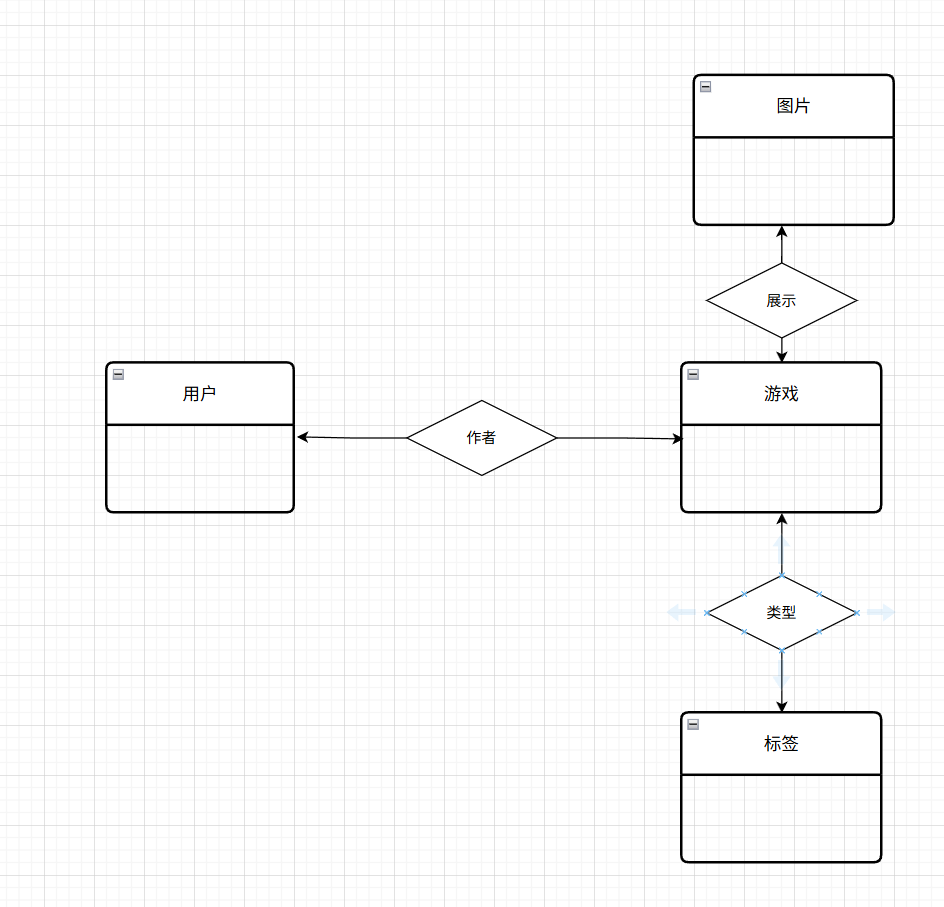
\includegraphics[width=0.8\textwidth]{dataset_ER.png}
  \caption{ER图}
\end{figure}
基于以上ER图,可以设计出系统需要的数据库表:
\begin{figure}[H]
  \centering
  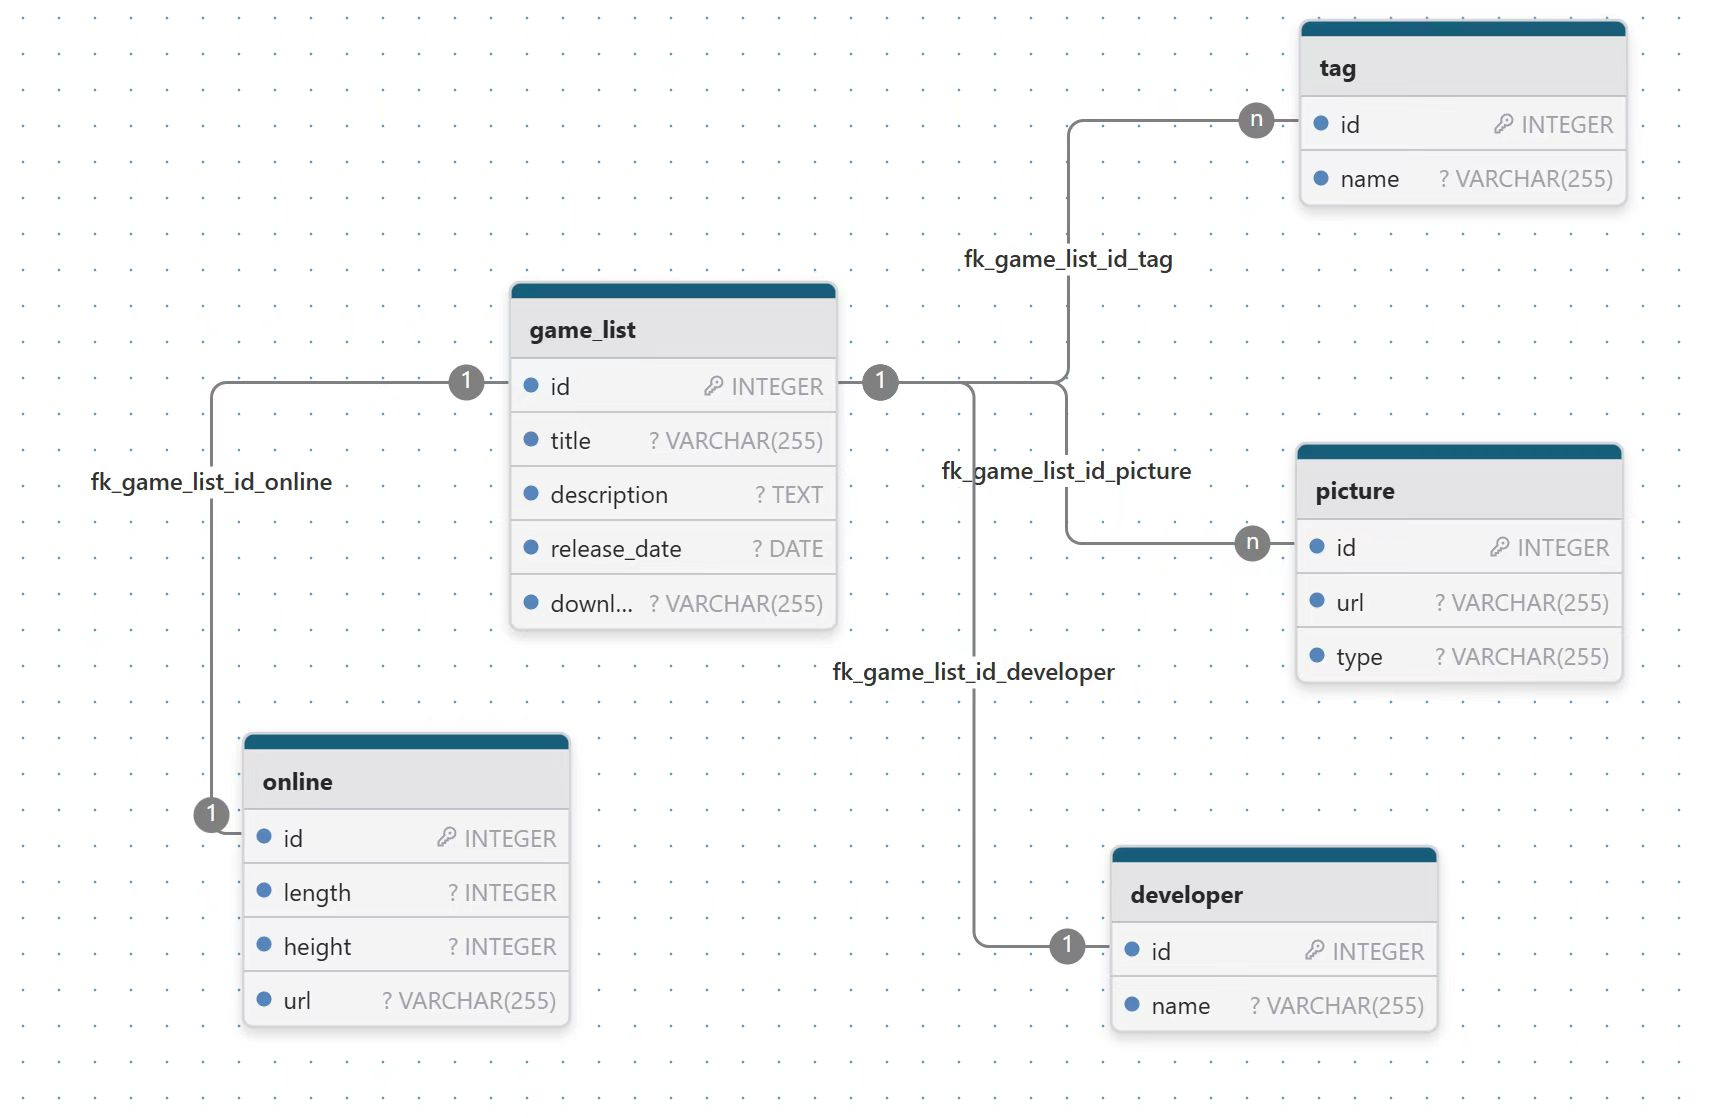
\includegraphics[width=0.8\textwidth]{dataset_metadata.jpg}
  \caption{数据库表}
\end{figure}

\section{客户端设计}

本次使用全栈客户端 Next.js 框架,其具备的拓展性可帮助打破单纯 “视图层” 的特性。
简单的 API Router 设计具备直接访问数据库的功能,但为了更好的分工安排,我们减轻全栈设计的复杂性, RESTful API 仍然由传统后端提供。
但在涉及用户权限控制时,仍然会使用 Next.js 的 API Router 进行更灵活、安全的路由处理。而如果使用了服务器端数据获取和渲染,则也应该使用服务器端动态渲染的形式。

\subsection{客户端架构}

主要采用组件式设计,组件化设计的好处在于可以将复杂的 UI 拆分成更小的、可重用的组件。每个组件都可以独立开发、测试和维护,从而提高了代码的可读性和可维护性。
组件化设计还可以提高开发效率,因为多个开发人员可以同时工作在不同的组件上,而不必担心相互之间的干扰。组件树示例如下:

\begin{figure}[H]
  \centering
  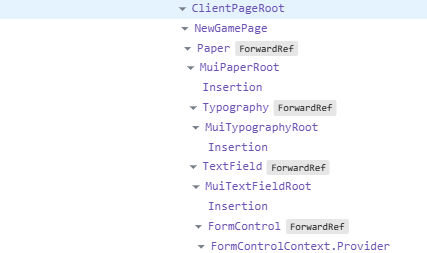
\includegraphics[width=0.8\textwidth]{Client-tree.png}
  \caption{组件树示例}
\end{figure}

\subsection{客户端路由}

Next.js 的路由系统是基于文件系统的,页面文件存放在 `app` 目录下,文件名即为路由路径。每个页面都是一个 React 组件,Next.js 会自动处理路由和页面渲染。

\begin{figure}[H]
  \centering
  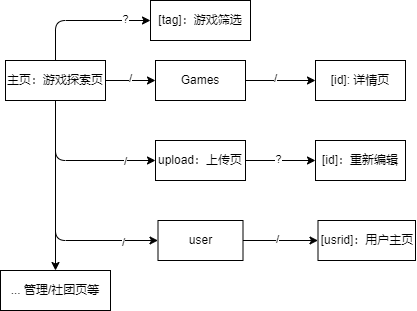
\includegraphics[width=0.8\textwidth]{Client-arch.png}
  \caption{目前的客户端路由}
\end{figure}


\subsection{渲染与缓存}

对于各部分的小块 data,采用视图和控制器分离的设计模式,以确保前端 model 的唯一性。而对于完整的页面,使用 Static Site Generation(增量静态再生)来进行渲染。
在正常情况下,设置 validate 字段为较长的时期,以始终持有 Full Route Cache 。 而在一定时间后,或有新游戏上传,资讯需要更新时,才使用细粒度较好的 revalidatePath 或 revalidateTag 来进行页面的增量构建。
这在极大减少客户端请求数目的同时,也能减轻服务器压力,并保证数据的实时性。

\begin{figure}[H]
  \centering
  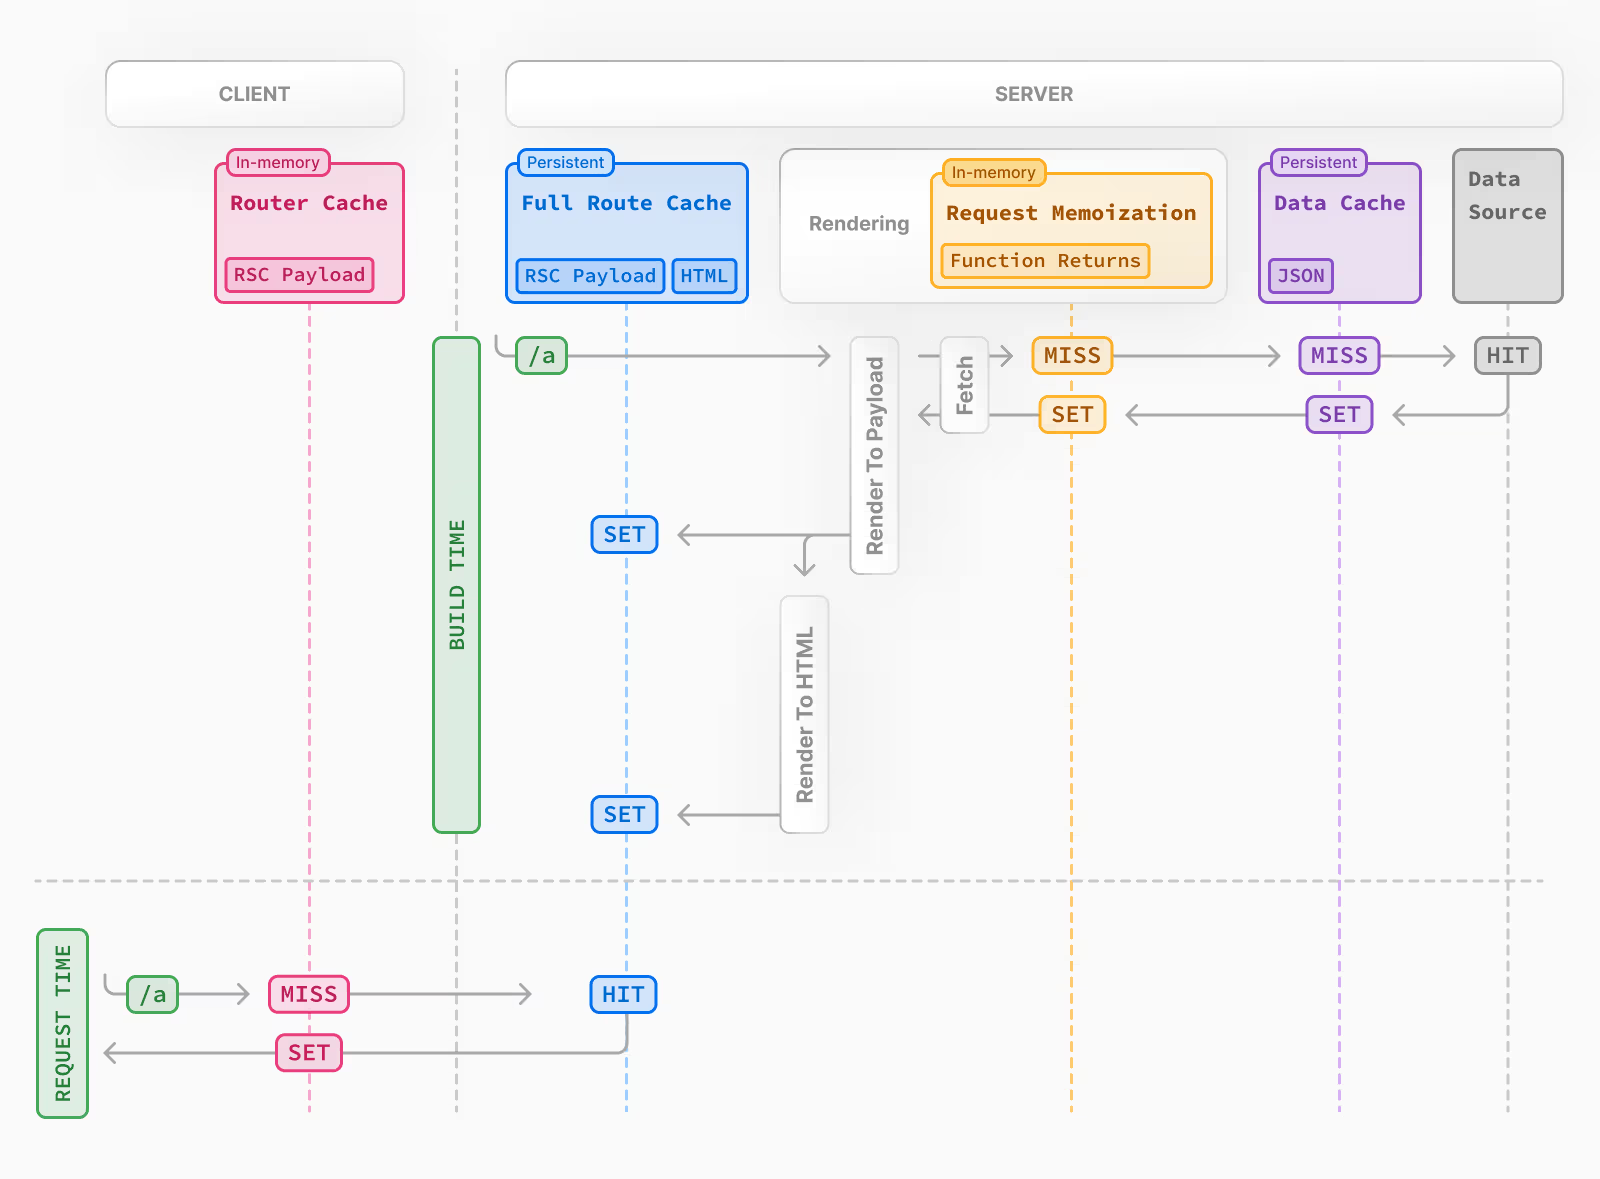
\includegraphics[width=0.8\textwidth]{Next-Cache.png}
  \caption{Next.js 数据缓存时序图}
\end{figure}

\section{界面原型}

本项目大量参考 \href{https://itch.io}{itch.io} 、\href{https://www.gcores.com/booom/game_lib}{BOOOM暴造} 等游戏资源分享网站
并专注于游戏资源上传和分享、评分功能,大量简化博客、活动宣传、关注、私聊等社区功能。因此界面原型也大致参考这些网站搭建。就算经验不足,也保证不大幅偏离 “最佳实践”。

以下标明 “参考” 的是参考网站的界面设计,其他的则是我们自己设计的界面原型。

\subsection{登录界面}

使用 UAuth2.0 协议登录,用户可以使用第三方账号(最好是zjuam)登录,因此没必要提供注册界面。

\subsection{主页/游戏探索页}


\subsection{游戏筛选页(参考)}

提供按照某种游戏 tag,比如 `Horror` 标签,或者发布时间、游玩平台进行筛选。后续将直接加到首页,便于筛选。
注意最终交付版本不提供价格/购买功能,因此也没有其筛选项。

\begin{figure}[H]
  \centering
  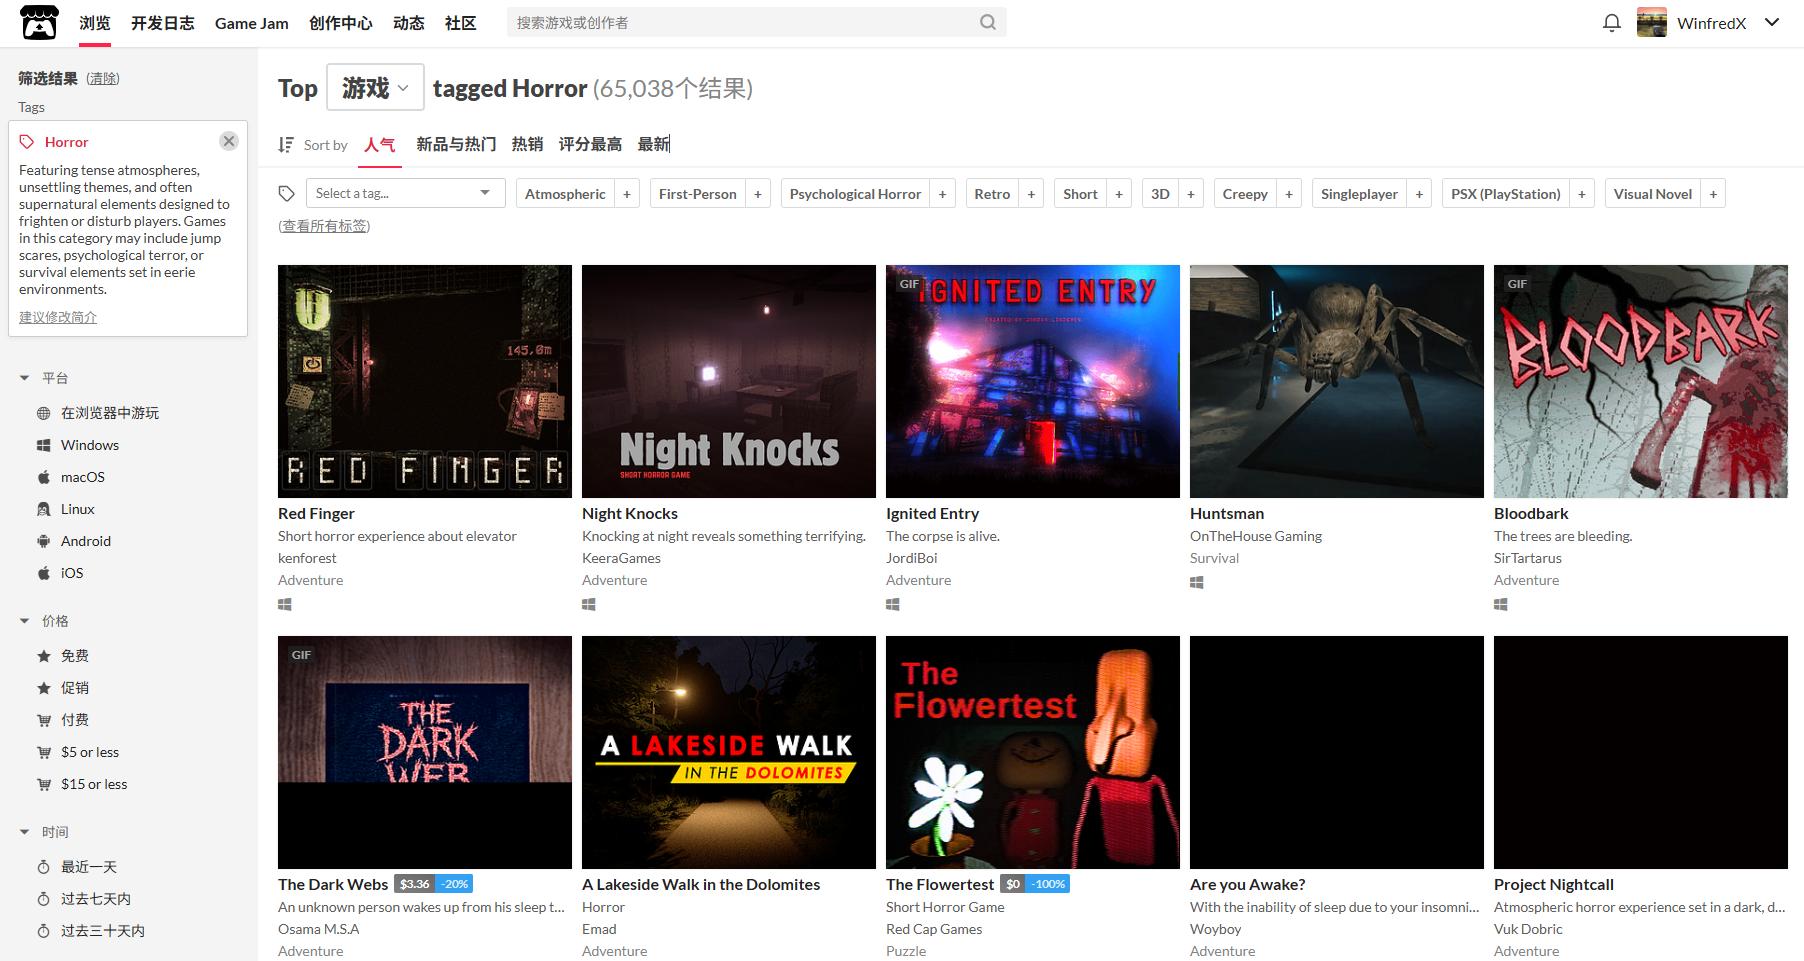
\includegraphics[width=0.8\textwidth]{UI-tagged.png}
  \caption{游戏探索页-按标签筛选}
\end{figure}

\subsection{游戏上传/编辑管理页}

重复利用该表单以实现游戏的上传和所有者/管理员的编辑功能。用户可以在该表单中上传游戏资源,填写游戏信息。

\begin{figure}[H]
  \centering
  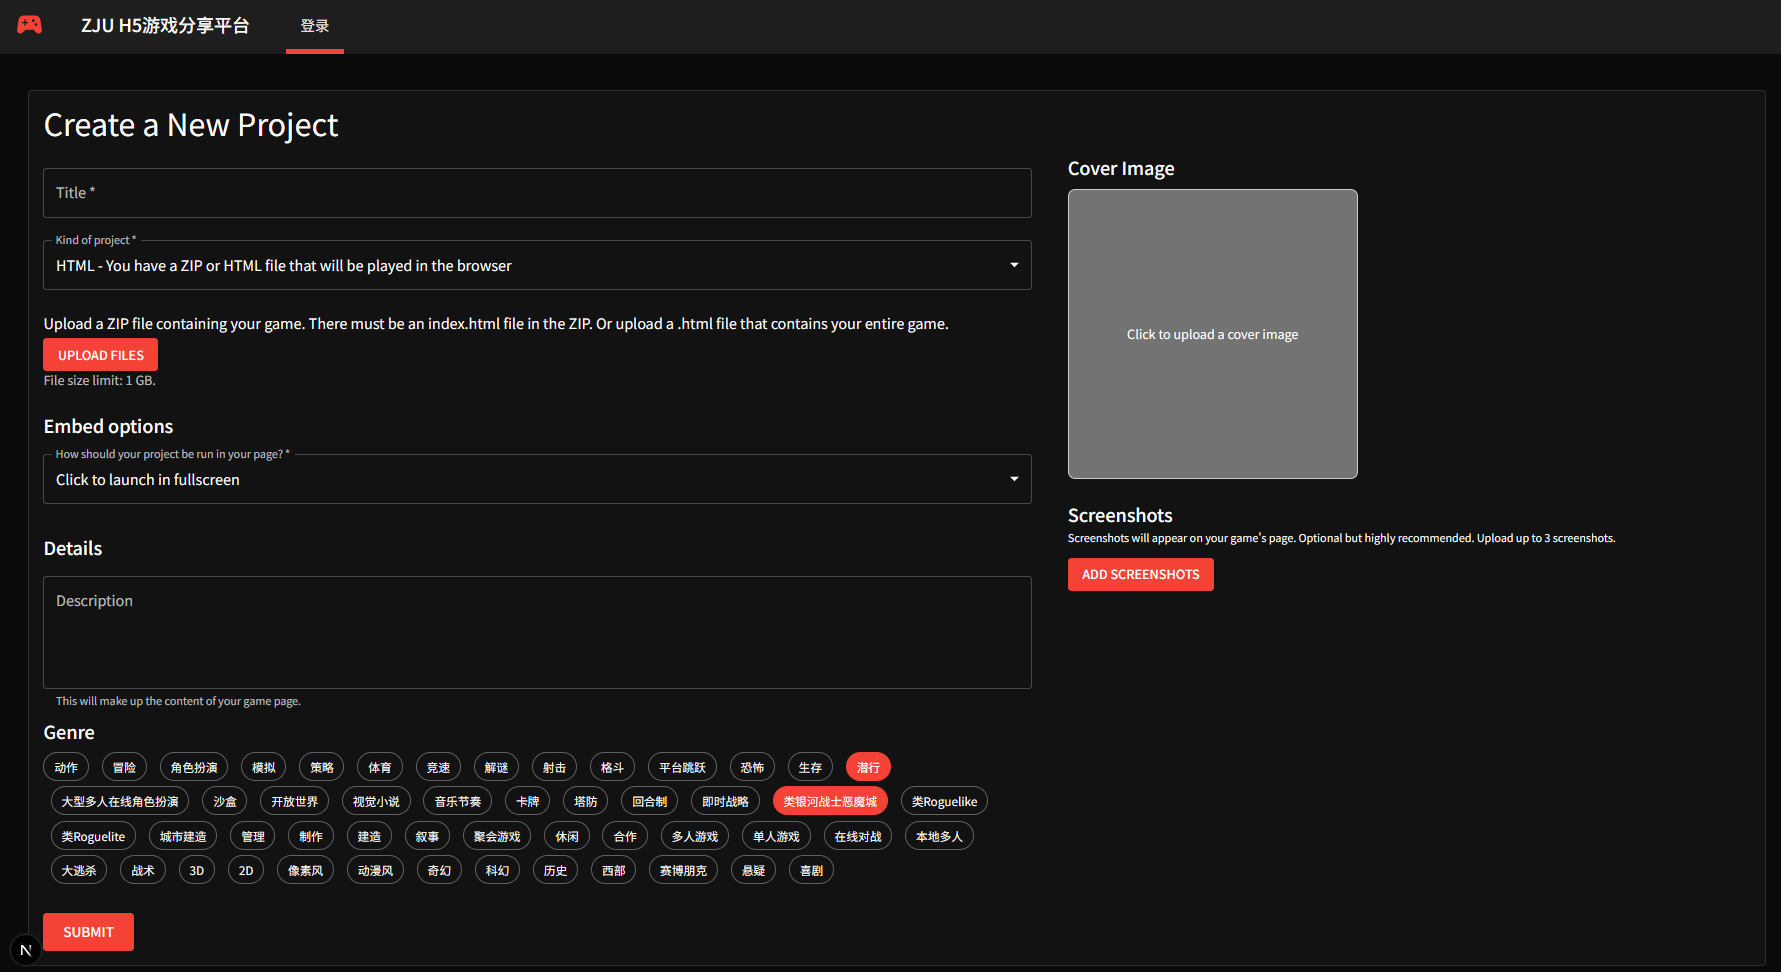
\includegraphics[width=0.8\textwidth]{UI-upload.png}
  \caption{游戏上传页}
\end{figure}


\subsection{游戏详情与进行页}

主要分为纵向两部分,第一个是游玩通道与详细信息,目前已经实现其设计,如果是在线游戏,那么最上方嵌入画布:

\begin{figure}[H]
  \centering
  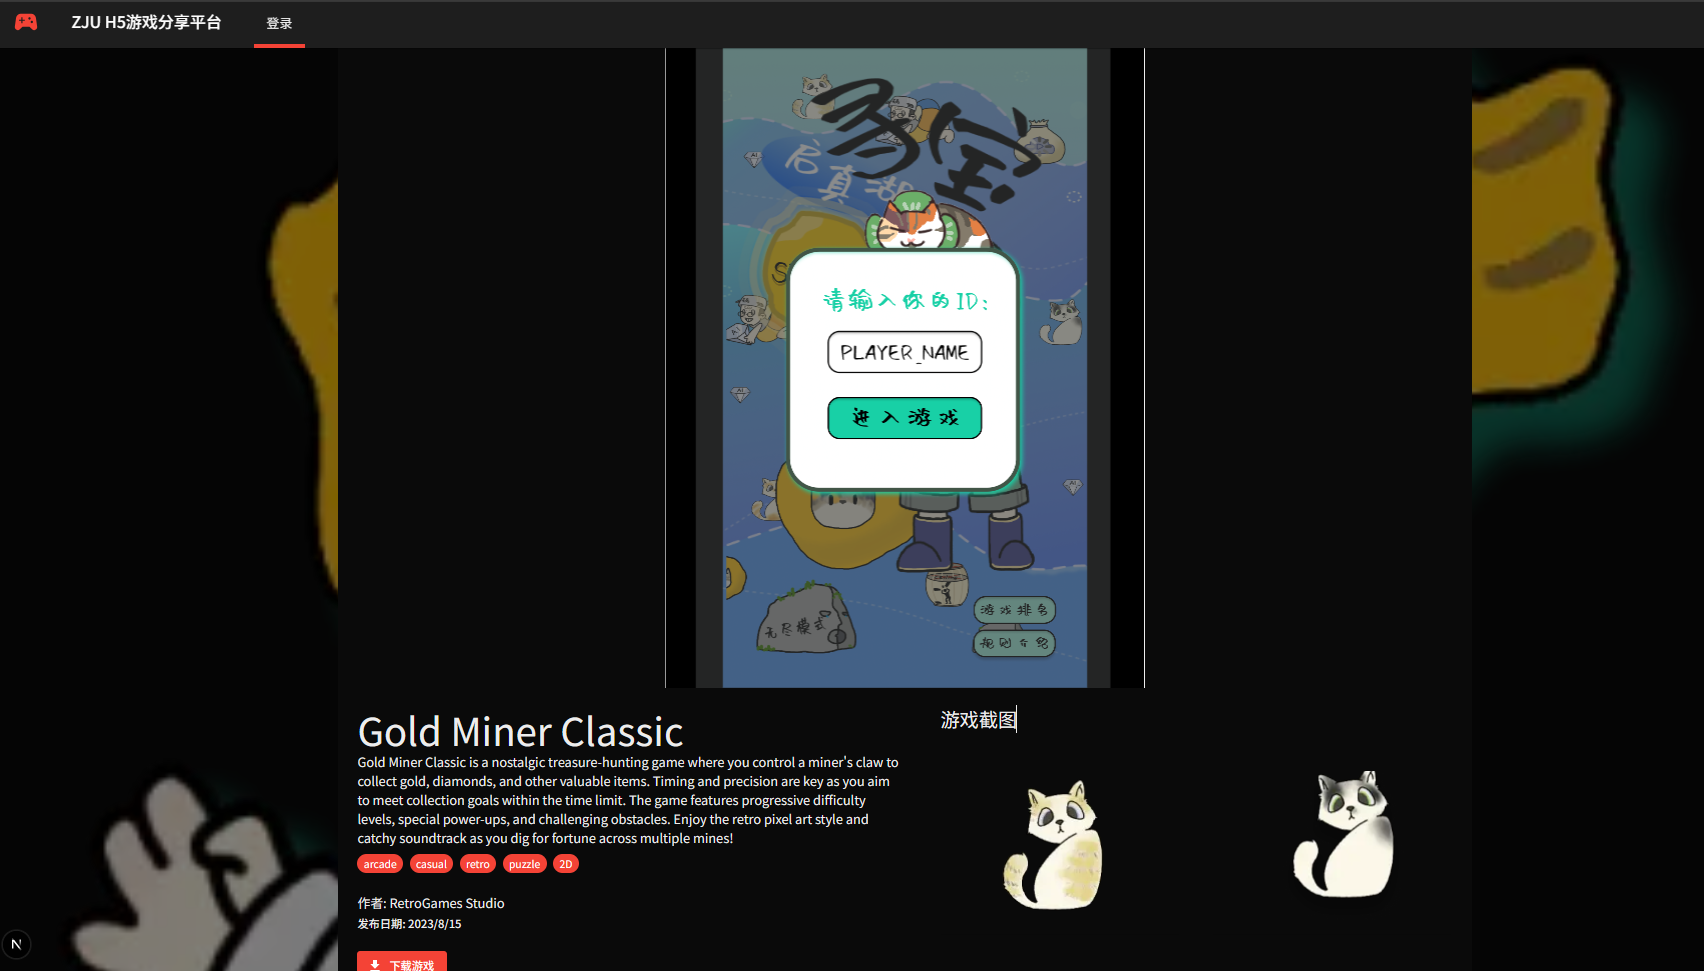
\includegraphics[width=0.8\textwidth]{UI-detailed.png}
  \caption{游戏详情页的游玩和介绍区}
\end{figure}


第二个是打分与评论区,评论区是 itch 网站参考图:


\begin{figure}[H]
  \centering
  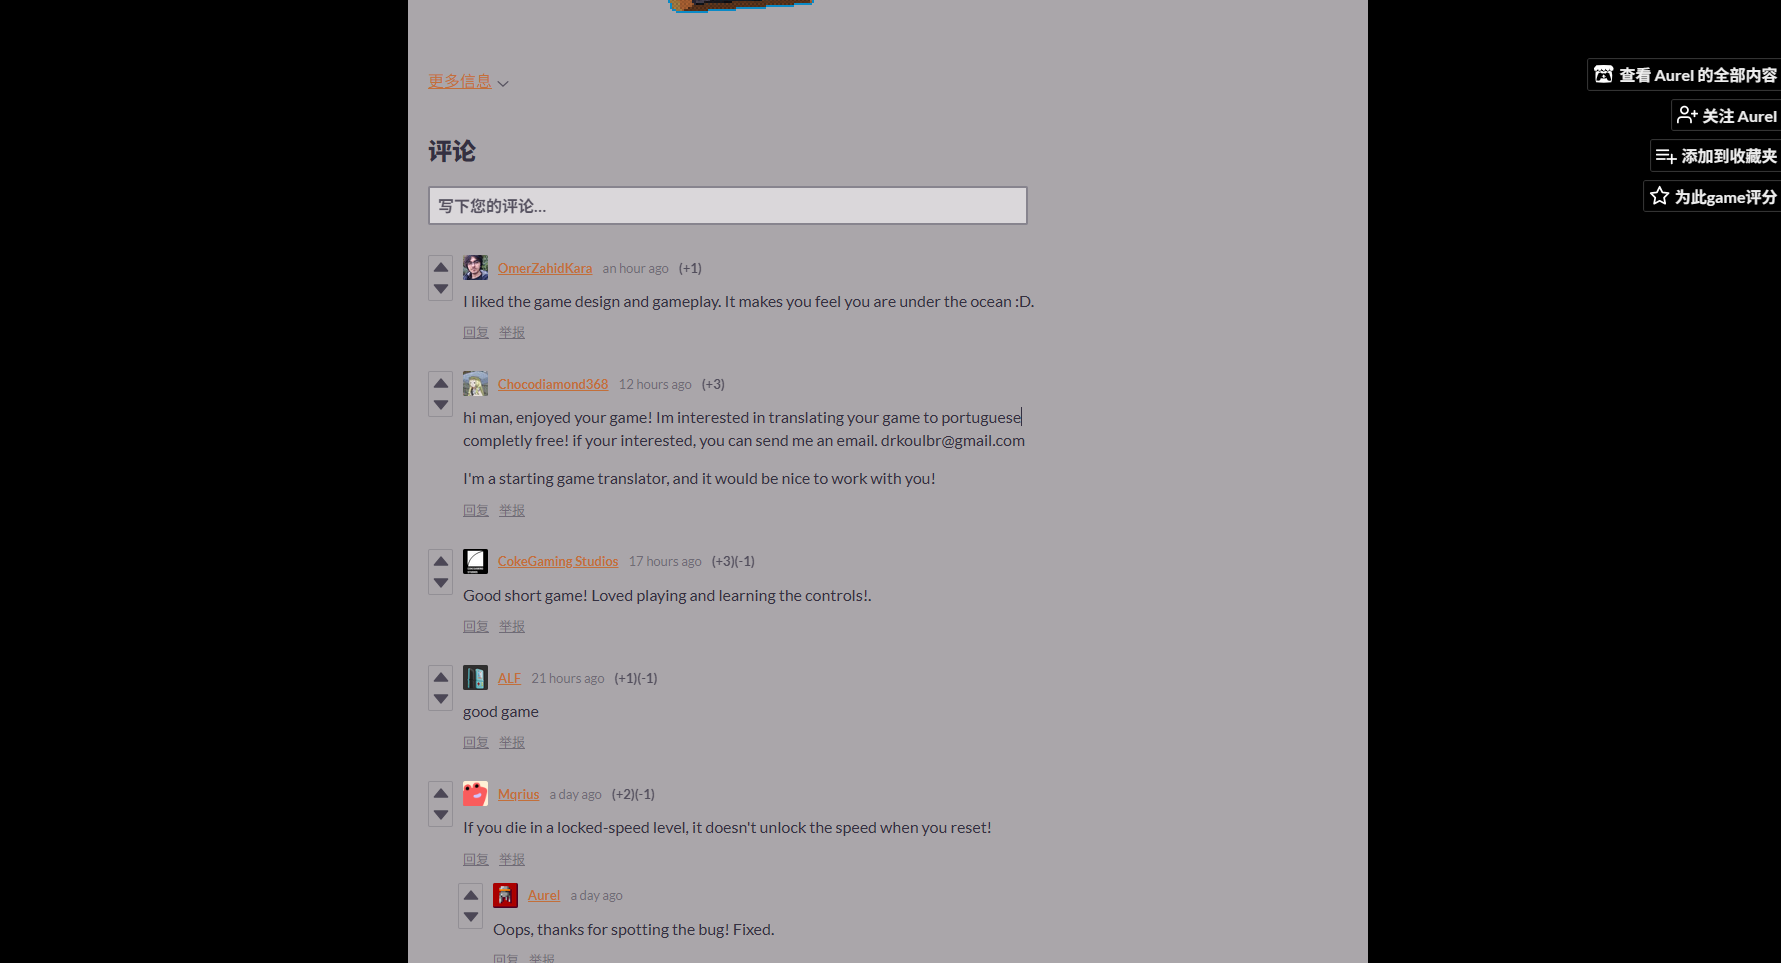
\includegraphics[width=0.8\textwidth]{UI-comment.png}
  \caption{游戏详情页的评论区}
\end{figure}

\subsection{个人信息页(参考)}

在 itch.io 这样创意性十足的网页中,个人信息页是可以灵活编辑其排版和显示内容,甚至可以手动插入 CSS 样式。
但最核心的功能还是个人联系方式和游戏制作列表的展示,简易版将在后续实现。

\begin{figure}[H]
  \centering
  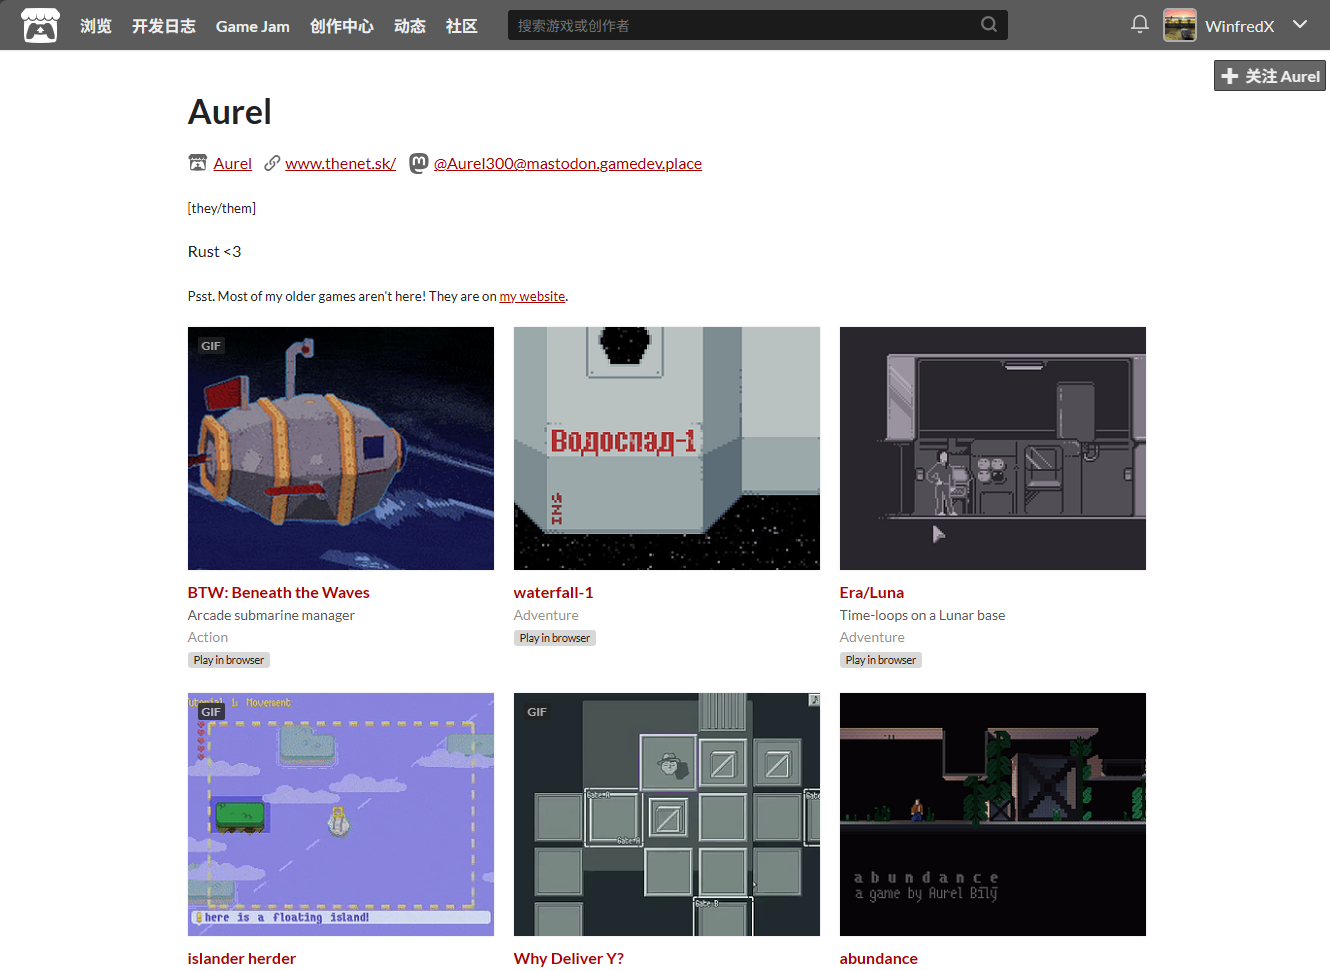
\includegraphics[width=0.8\textwidth]{UI-profile.png}
  \caption{itch.io 的个人信息页}
\end{figure}


\subsection{管理员后台}


\end{document}